\documentclass[../../../main]{subfiles}
\begin{document}

\section{実験4}
\begin{figure}
	\centering
	\begin{subfigure}{0.45\textwidth}
		\centering
		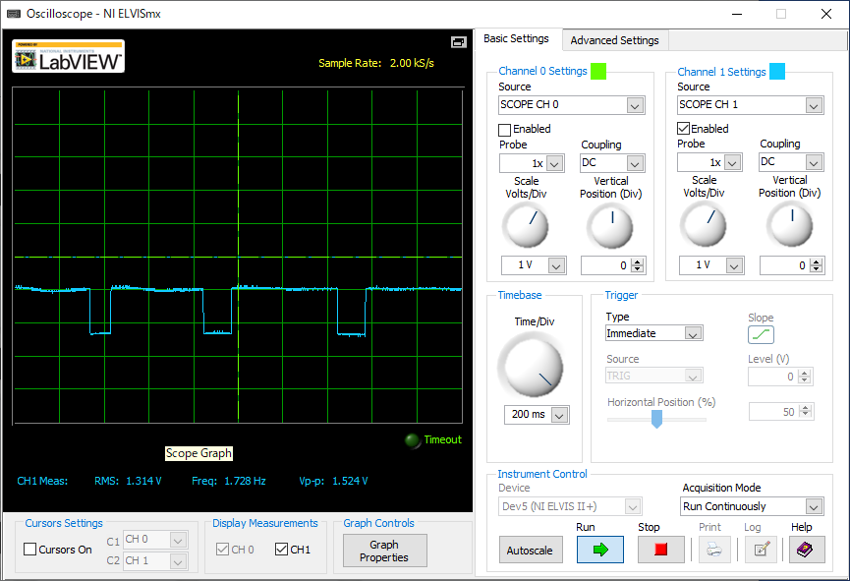
\includegraphics[width=\textwidth]{src/figures/exp4/led.png}
		\subcaption{太陽電池}
		\label{subfig:exp4-led}
	\end{subfigure}
	\begin{subfigure}{0.45\textwidth}
		\centering
		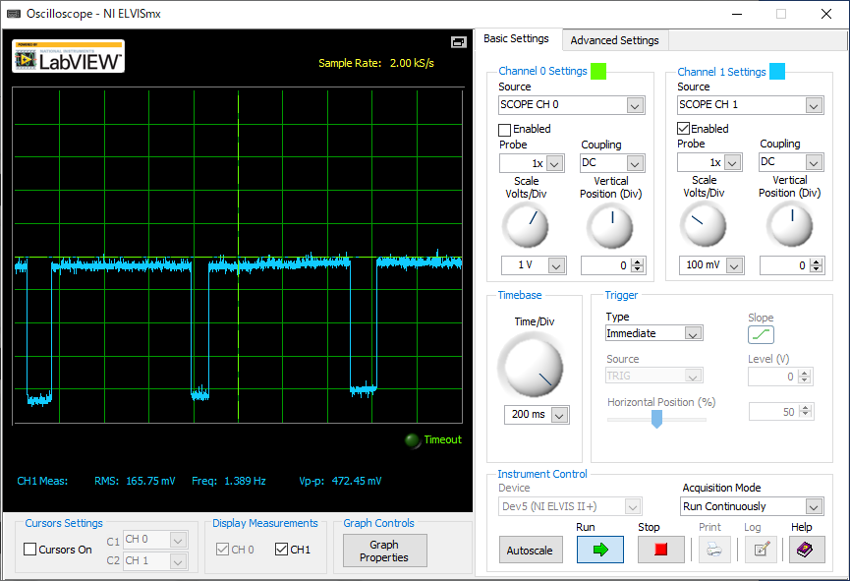
\includegraphics[width=\textwidth]{src/figures/exp4/photo-diode.png}
		\subcaption{フォトダイオード}
		\label{subfig:exp4-photo-diode}
	\end{subfigure}
	\caption{LEDライトを点灯させたときの出力波形}\label{fig:exp4-led}
\end{figure}

\begin{figure}
	\centering
	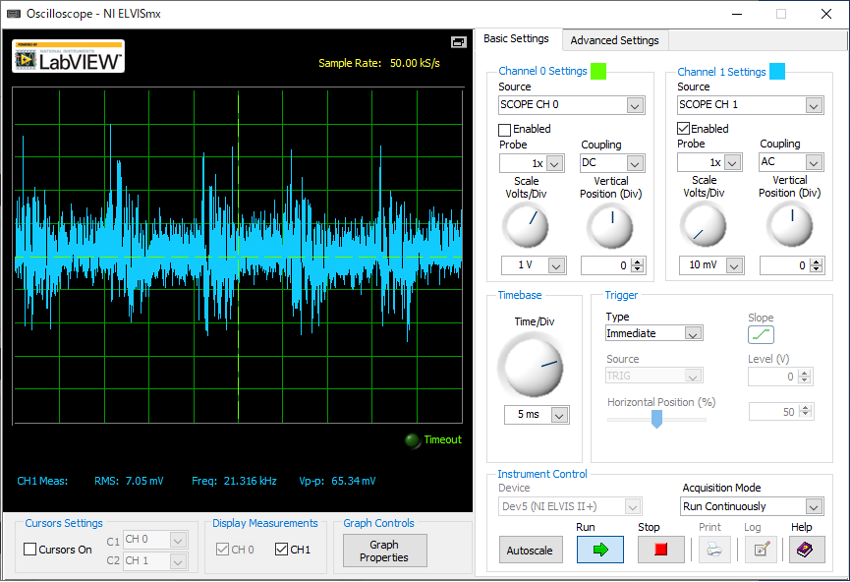
\includegraphics[width=0.6\linewidth]{src/figures/exp4/f-lamp.png}
	\caption{実験室の照明(蛍光灯)下での出力波形}\label{fig:exp4-f-lamp}
\end{figure}


\clearpage
\section{実験5}
\begin{figure}[!htb]
    \centering
    \centering
    \begin{subfigure}{0.48\linewidth}
        \centering
        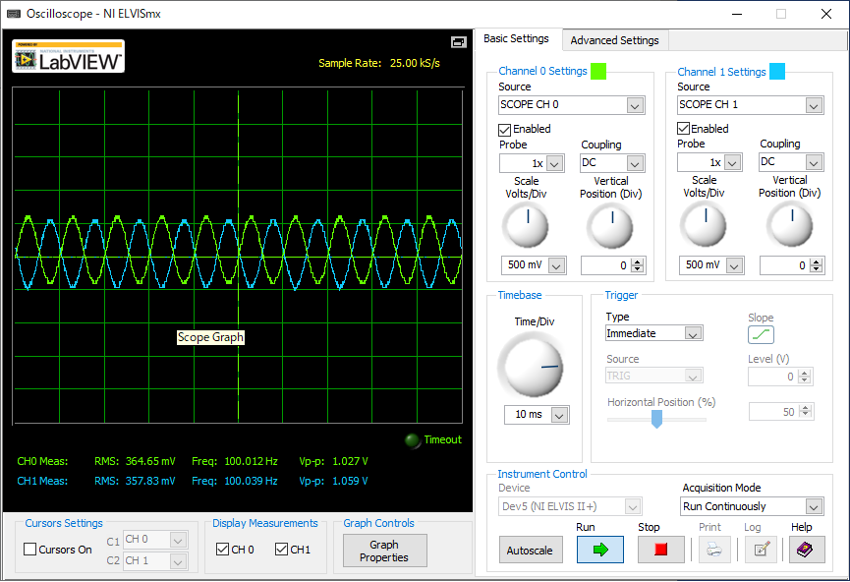
\includegraphics[width=0.8\linewidth]{src/figures/exp5/amp-10k.png}
        \subcaption{$R=\SI{10}{k\ohm}$のとき}\label{fig:exp5-raw-10k}
    \end{subfigure}
    \begin{subfigure}{0.48\linewidth}
        \centering
        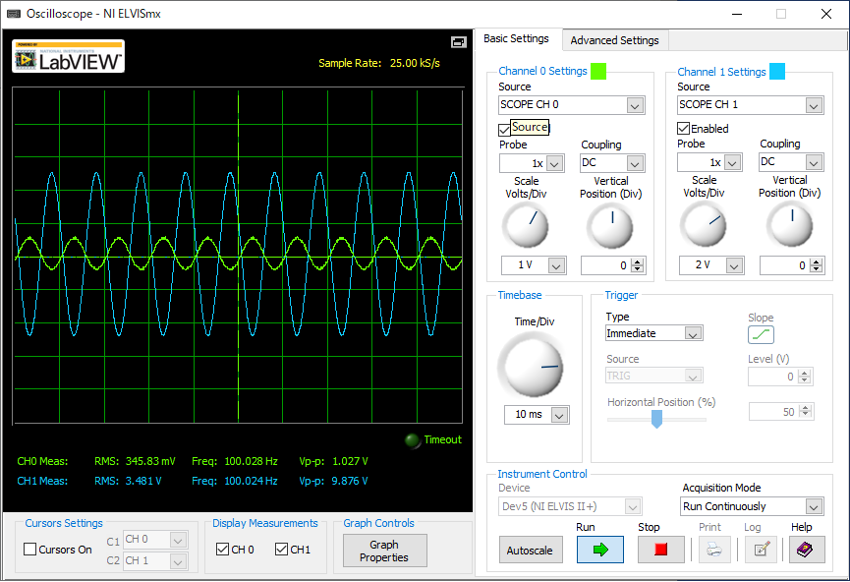
\includegraphics[width=0.8\linewidth]{src/figures/exp5/amp-1k.png}
        \subcaption{$R=\SI{1}{k\ohm}$のとき}\label{fig:exp5-raw-1k}
    \end{subfigure}
    \caption{実験5 オペアンプの出力波形}\label{fig:exp5-raw}
\end{figure}


\clearpage
\section{実験6}
\begin{figure}[!htb]
	\centering
	\begin{subfigure}{0.48\linewidth}
		\centering
		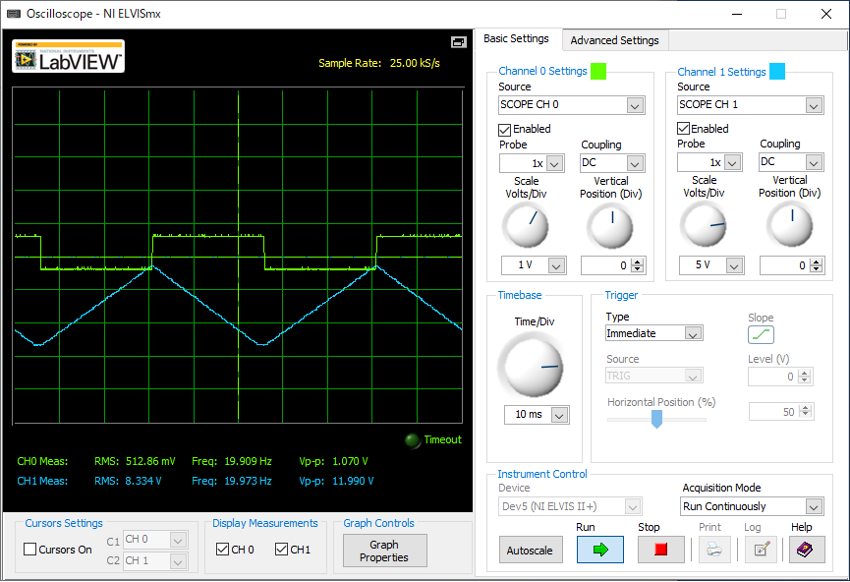
\includegraphics[width=0.8\linewidth]{src/figures/exp6/int.png}
		\subcaption{積分回路に矩形波を入力した時の出力}\label{fig:exp6-int}
	\end{subfigure}
	\begin{subfigure}{0.48\linewidth}
		\centering
		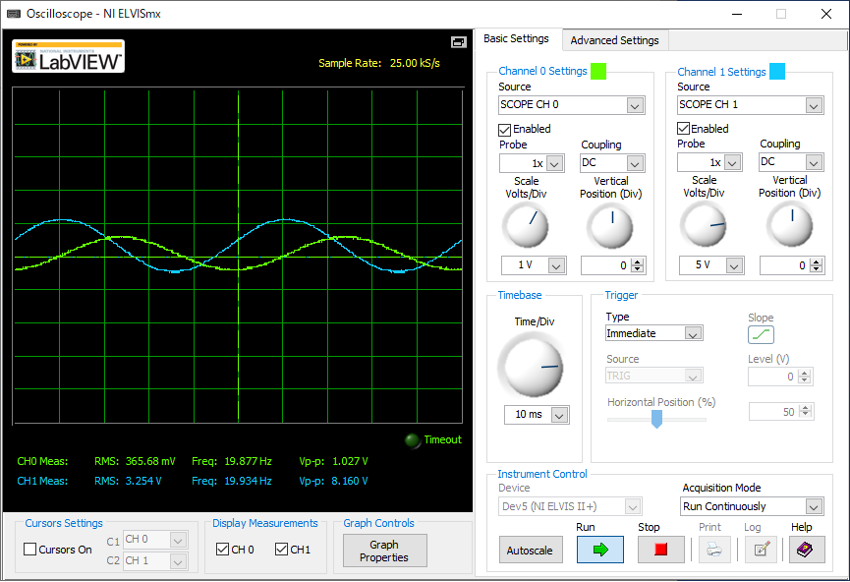
\includegraphics[width=0.8\linewidth]{src/figures/exp6/int-res-sin.png}
		\subcaption{不完全積分回路に正弦波を入力したときの出力}\label{fig:exp6-int-res-sin}
	\end{subfigure}
	\begin{subfigure}{0.48\linewidth}
		\centering
		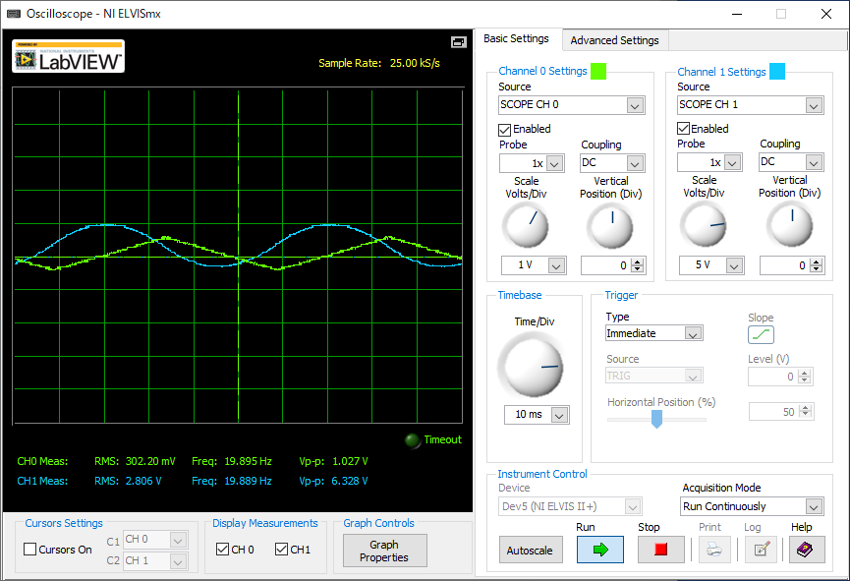
\includegraphics[width=0.8\linewidth]{src/figures/exp6/int-res-tri.png}
		\subcaption{不完全積分回路に三角波を入力したときの出力}\label{fig:exp6-int-res-tri}
	\end{subfigure}
	\begin{subfigure}{0.48\linewidth}
		\centering
		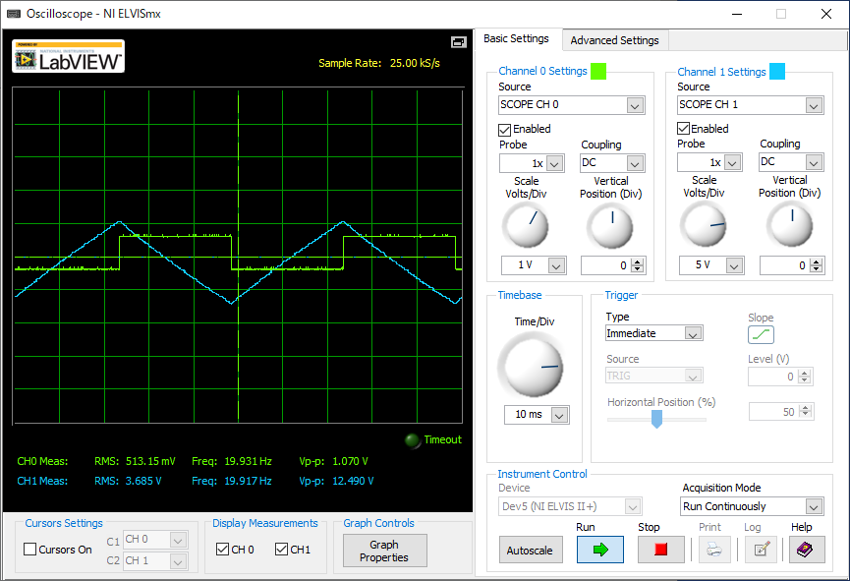
\includegraphics[width=0.8\linewidth]{src/figures/exp6/int-res-sq.png}
		\subcaption{不完全積分回路に矩形波を入力したときの出力}\label{fig:exp6-int-res-sq}
	\end{subfigure}
	\caption{実験6で撮影した画像}\label{fig:exp6-raw}
\end{figure}


\clearpage
\section{実験7}
\begin{figure}
    \centering
    \begin{subfigure}{0.45\textwidth}
        \centering
        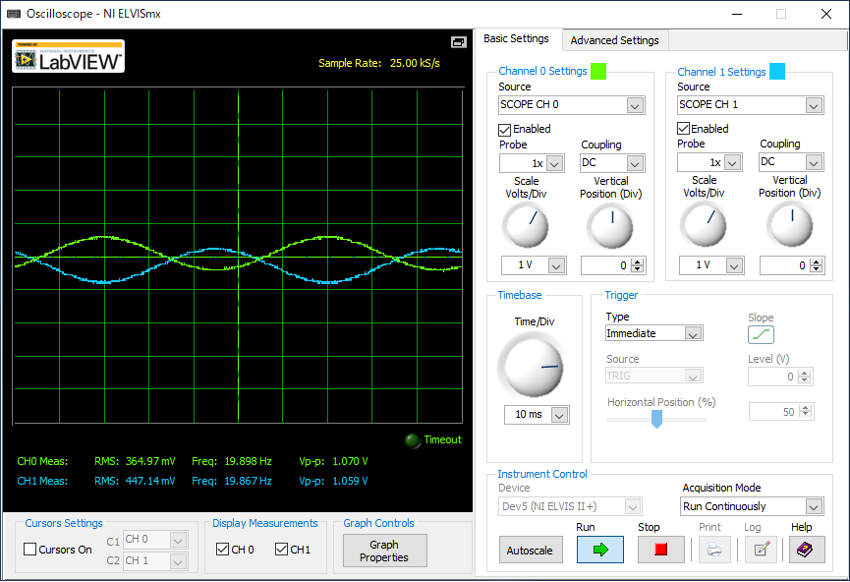
\includegraphics[width=0.8\linewidth]{src/figures/exp7/sum-0.png}
        \subcaption{VPS: \SI{0}{V}}\label{fig:exp7-raw-0}
    \end{subfigure}
    \begin{subfigure}{0.45\textwidth}
        \centering
        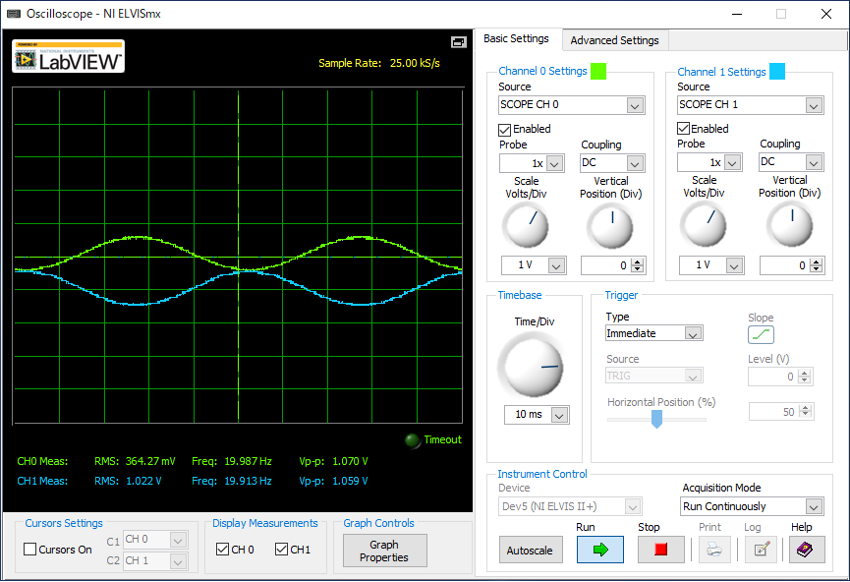
\includegraphics[width=0.8\linewidth]{src/figures/exp7/sum-1.png}
        \subcaption{VPS: \SI{1}{V}}\label{fig:exp7-raw-1}
    \end{subfigure}
    \begin{subfigure}{0.45\textwidth}
        \centering
        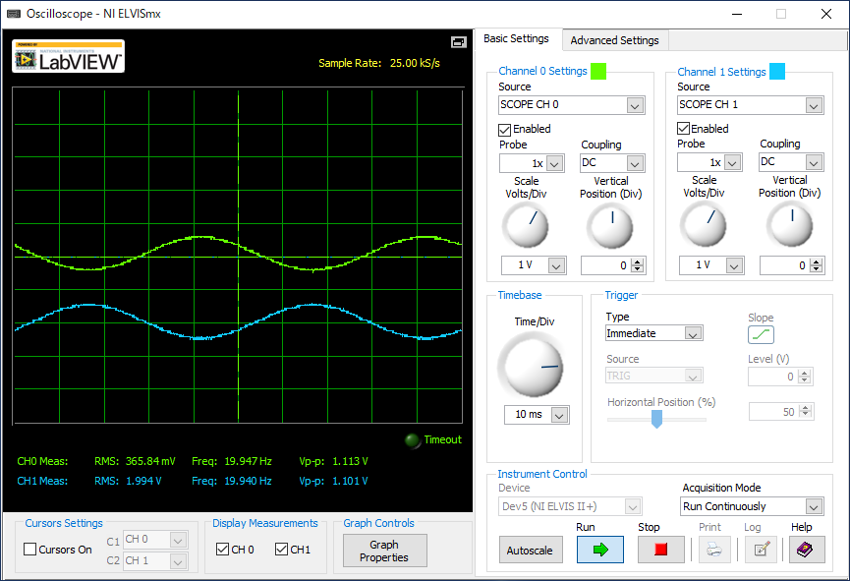
\includegraphics[width=0.8\linewidth]{src/figures/exp7/sum-2.png}
        \subcaption{VPS: \SI{2}{V}}\label{fig:exp7-raw-2}
    \end{subfigure}
    \caption{加算回路の出力波形}\label{fig:exp7-raw}
\end{figure}


\clearpage
\section{実験8}
\begin{figure}
	\centering
	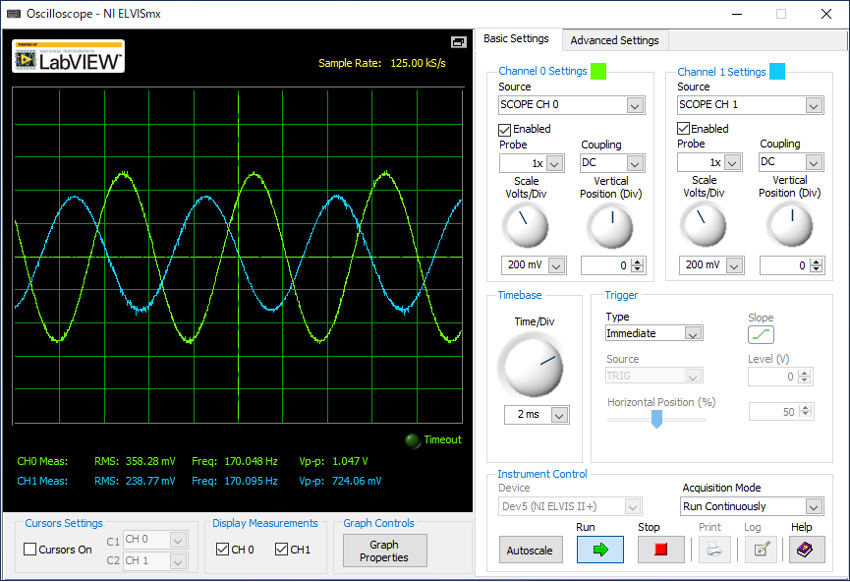
\includegraphics[width=0.8\linewidth]{src/figures/exp8/low-pass.png}
	\caption{ローパスフィルターのカットオフ周波数における波形}\label{fig:exp8-raw-cutoff}
\end{figure}

\begin{figure}
	\centering
	\begin{subfigure}{0.8\linewidth}
		\centering
		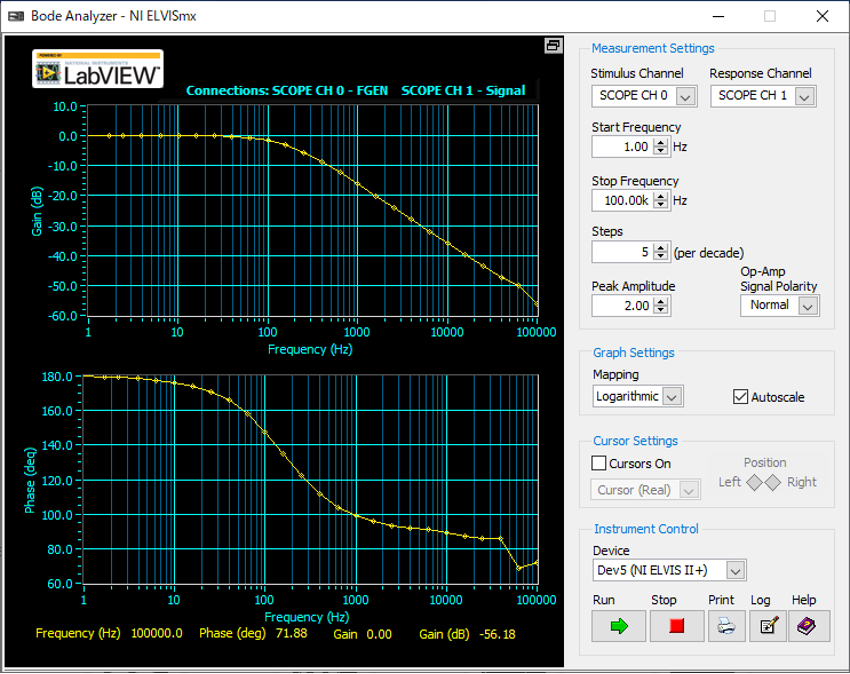
\includegraphics[width=0.8\linewidth]{src/figures/exp8/low-pass-bode-10k.png}
		\subcaption{$R_1=\SI{10}{k\ohm}$}
	\end{subfigure}
	\begin{subfigure}{0.8\linewidth}
		\centering
		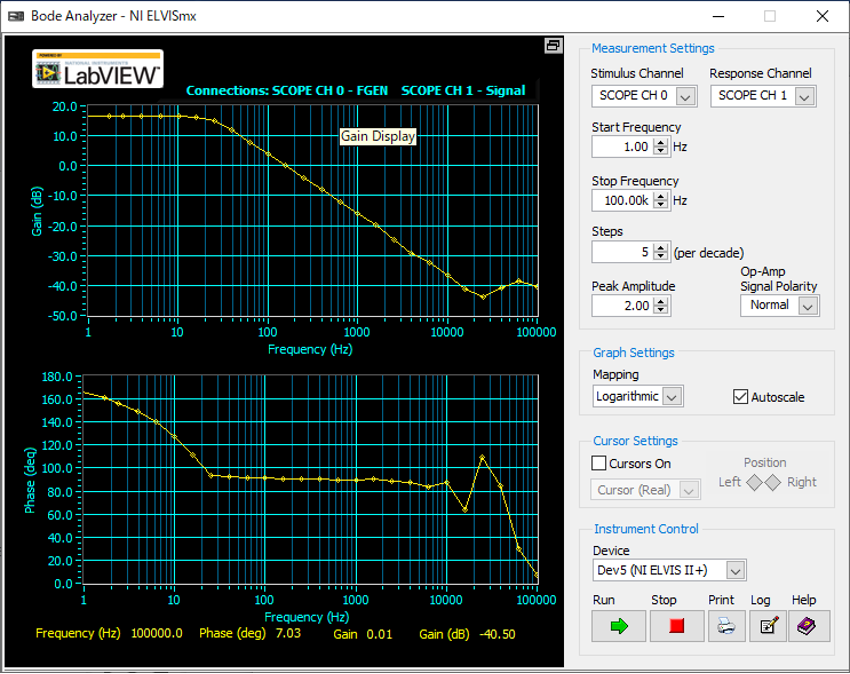
\includegraphics[width=0.8\linewidth]{src/figures/exp8/low-pass-bode-1m.png}
		\subcaption{$R_1=\SI{1}{M\ohm}$}
	\end{subfigure}
	\caption{ローパスフィルターのボード線図}\label{fig:exp8-bode}
\end{figure}


\clearpage
\section{実験9}
\begin{figure}
	\centering
	\begin{subfigure}{0.8\textwidth}
		\centering
		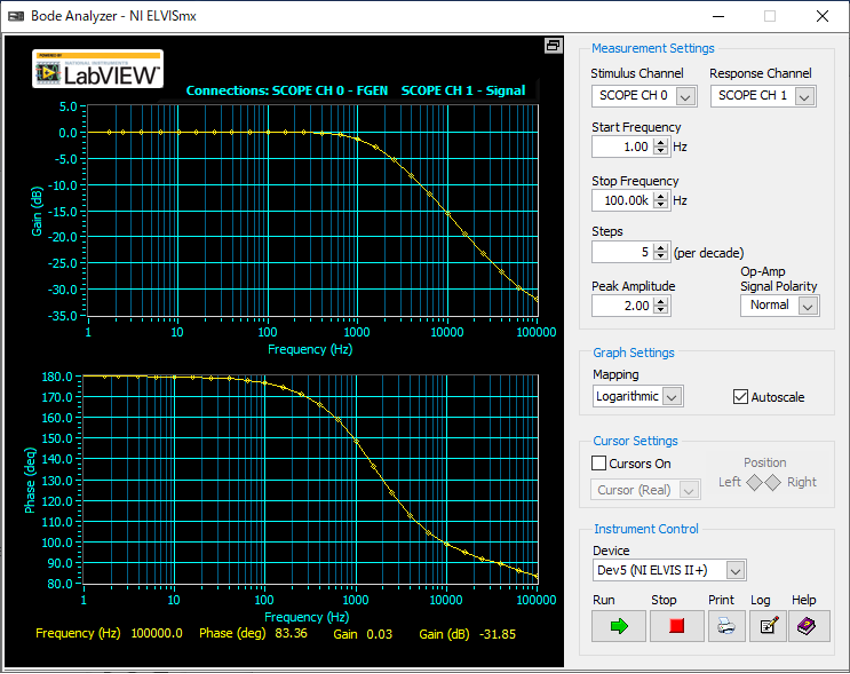
\includegraphics[width=0.8\linewidth]{src/figures/exp9/ope2-bode.png}
		\subcaption{オペアンプ2を用いたローパスフィルターのボード線図}\label{subfig:exp9-ope2-bode}
	\end{subfigure}
	\begin{subfigure}{0.8\textwidth}
		\centering
		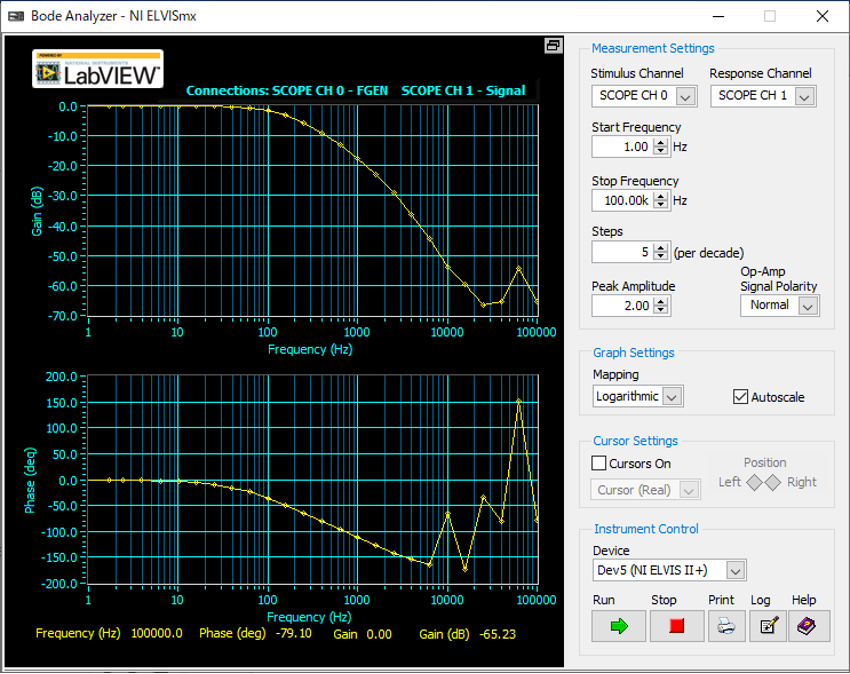
\includegraphics[width=0.8\linewidth]{src/figures/exp9/ope12-bode.png}
		\subcaption{オペアンプ1とオペアンプ2を継続接続したローパスフィルターのボード線図}\label{subfig:exp9-ope2-ope1-bode}
	\end{subfigure}
	\caption{実験9のボード線図}\label{fig:exp9-bode}
\end{figure}


\clearpage
\section{実験10}
\subsection*{バンドパスフィルタとローパスフィルターのボード線図}
\begin{figure}{!h}
	\centering
	\begin{subfigure}{0.8\linewidth}
		\centering
		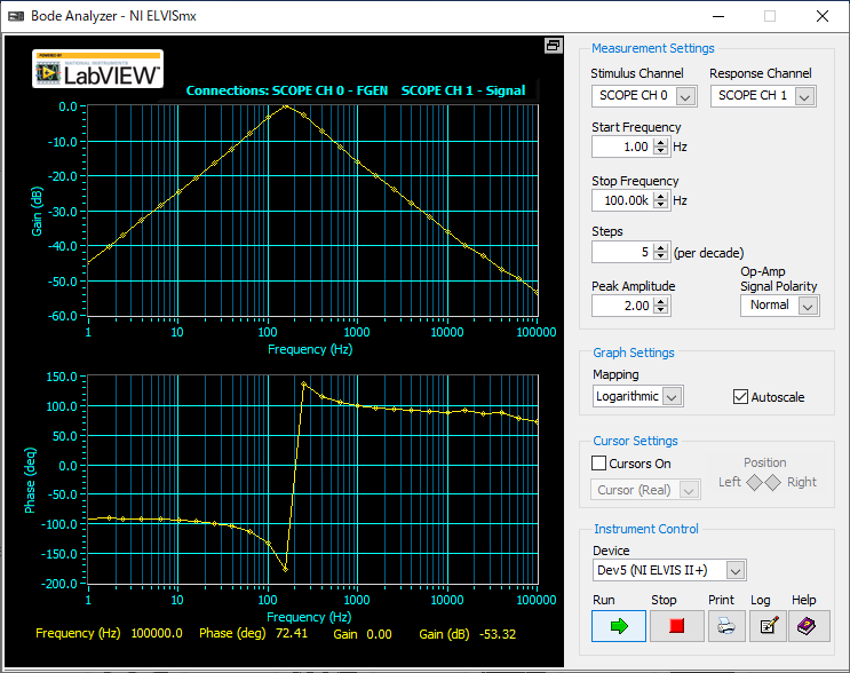
\includegraphics[width=0.8\linewidth]{src/figures/exp10/10k-low-bode.png}
		\subcaption{$R_1=\SI{10}{k\ohm}$のローパスフィルタのボード線図}\label{fig:exp10-10k-low-bode}
	\end{subfigure}
	\begin{subfigure}{0.8\linewidth}
		\centering
		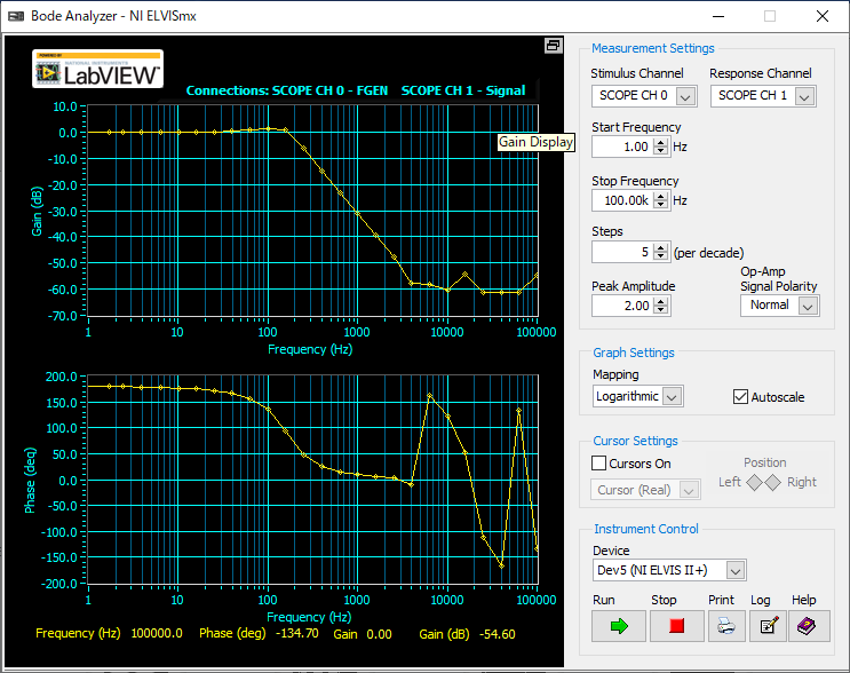
\includegraphics[width=0.8\linewidth]{src/figures/exp10/10k-band-bode.png}
		\subcaption{$R_1=\SI{10}{k\ohm}$のバンドパスフィルタのボード線図}\label{fig:exp10-10k-band-bode}
	\end{subfigure}
\end{figure}
\begin{figure}
	\centering
	\begin{subfigure}{0.8\linewidth}
		\addtocounter{subfigure}{2}
		\centering
		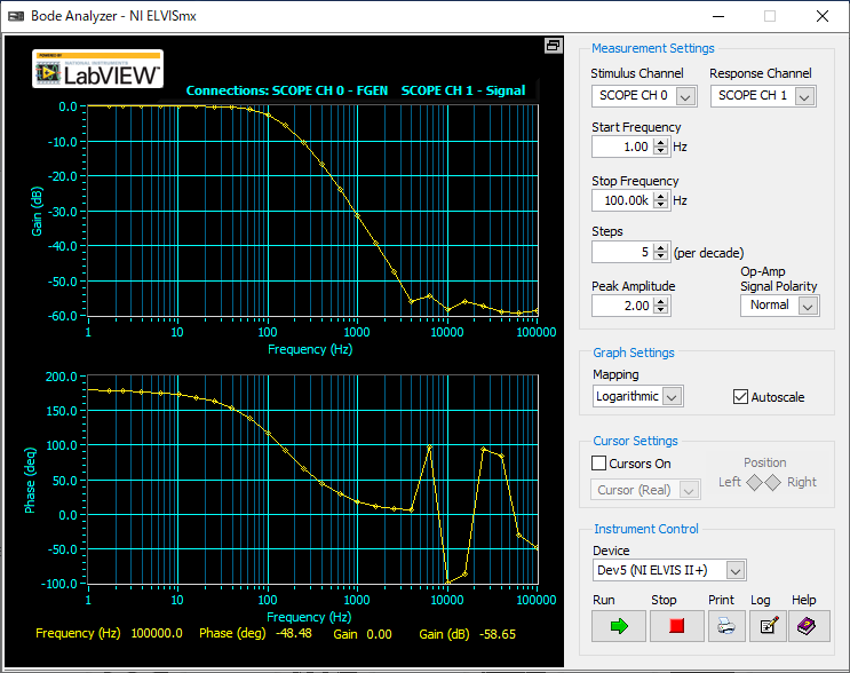
\includegraphics[width=0.8\linewidth]{src/figures/exp10/5k-band-bode.png}
		\subcaption{$R_1=\SI{5}{k\ohm}$のバンドパスフィルタのボード線図}\label{fig:exp10-5k-band-bode}
	\end{subfigure}
	\begin{subfigure}{0.8\linewidth}
		\centering
		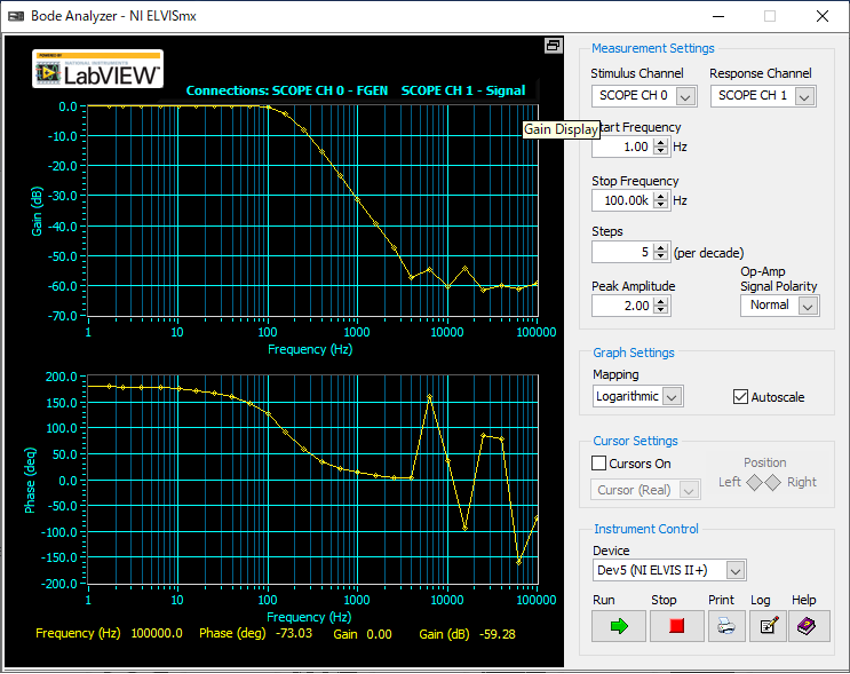
\includegraphics[width=0.8\linewidth]{src/figures/exp10/7k-band-bode.png}
		\subcaption{$R_1=\SI{7}{k\ohm}$のバンドパスフィルタのボード線図}\label{fig:exp10-7k-band-bode}
	\end{subfigure}
\end{figure}
\begin{figure}
	\centering
	\begin{subfigure}{0.8\linewidth}
		\addtocounter{subfigure}{4}
		\centering
		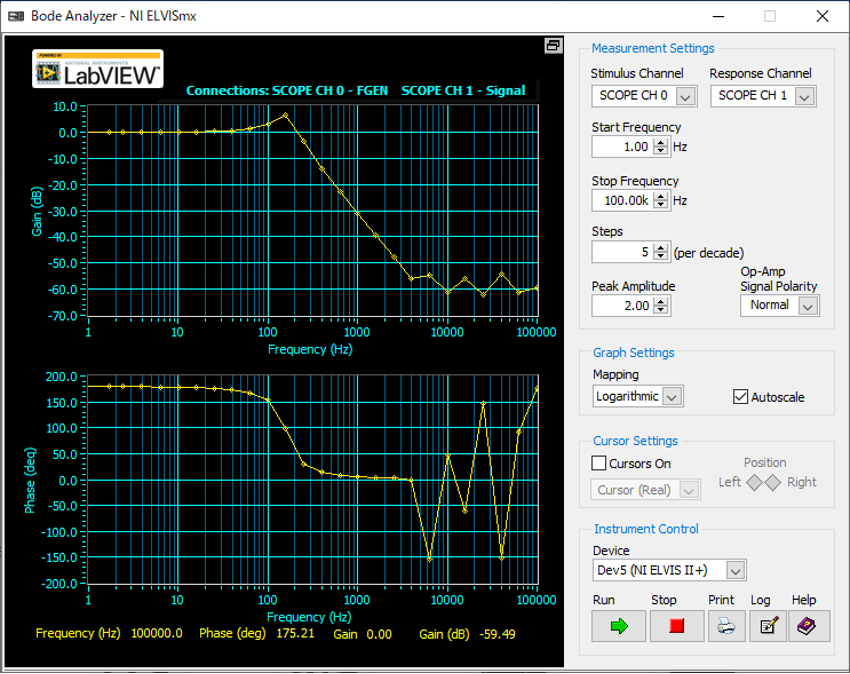
\includegraphics[width=0.8\linewidth]{src/figures/exp10/20k-band-bode.png}
		\subcaption{$R_1=\SI{20}{k\ohm}$のバンドパスフィルタのボード線図}\label{fig:exp10-20k-band-bode}
	\end{subfigure}
	\caption{実験10で作成したバイカット型フィルタのボード線図}\label{fig:exp10-bode}
\end{figure}


\clearpage
\subsection*{バンドパスフィルタの出力波形}
\begin{figure}
	\centering
	\begin{subfigure}{0.8\linewidth}
		\centering
		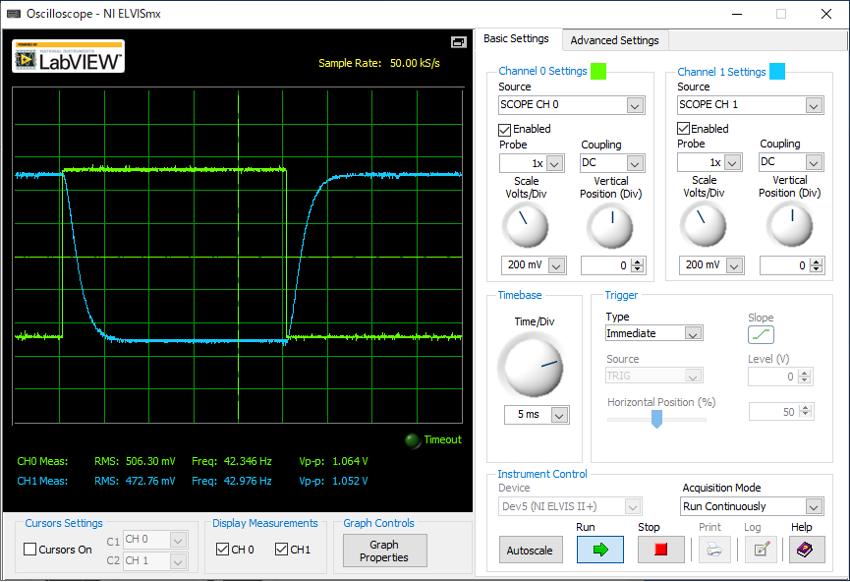
\includegraphics[width=0.8\linewidth]{src/figures/exp10/5k-low-sq.png}
		\subcaption{\SI{5}{k\ohm}でのバンドパスフィルタの出力波形}
	\end{subfigure}
	\begin{subfigure}{0.8\linewidth}
		\centering
		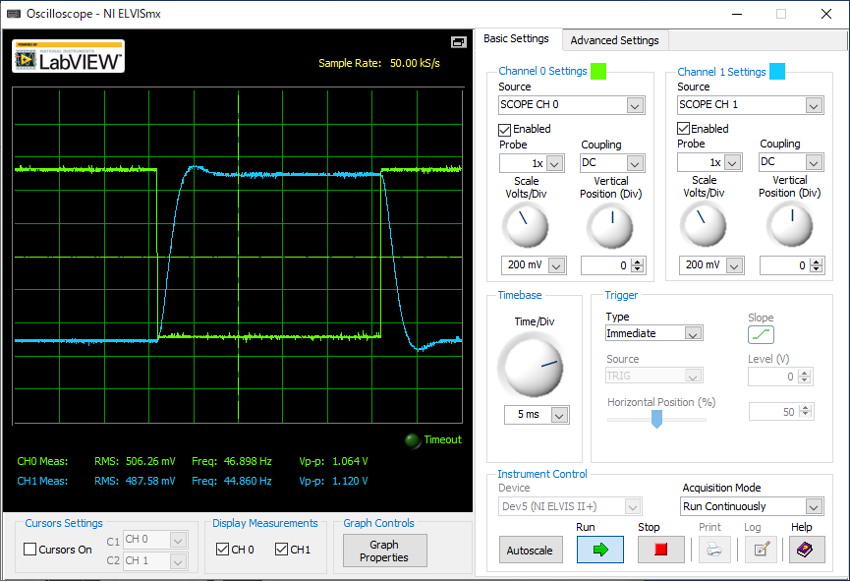
\includegraphics[width=0.8\linewidth]{src/figures/exp10/7k-low-sq.png}
		\subcaption{\SI{7}{k\ohm}でのバンドパスフィルタの出力}
	\end{subfigure}
\end{figure}
\begin{figure}
	\centering
	\begin{subfigure}{0.8\linewidth}
		\addtocounter{subfigure}{2}
		\centering
		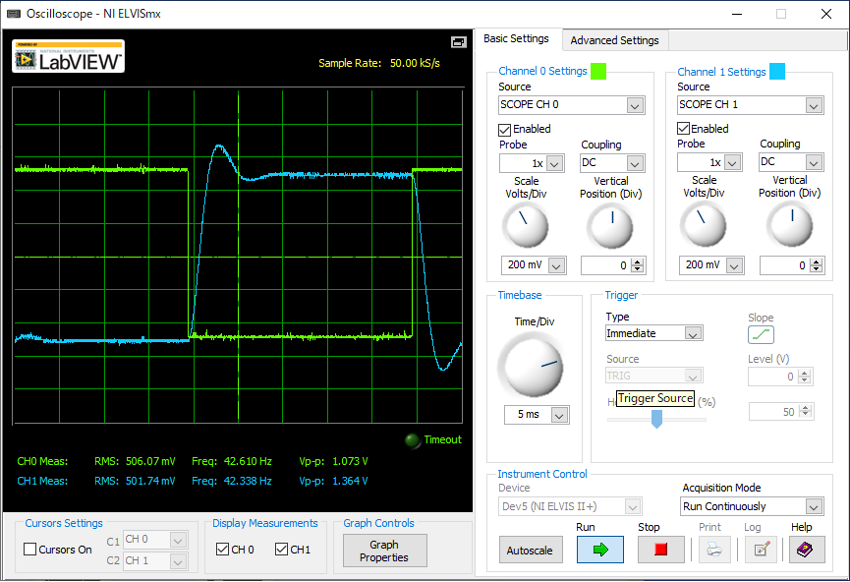
\includegraphics[width=0.8\linewidth]{src/figures/exp10/10k-low-sq.png}
		\subcaption{\SI{10}{k\ohm}でのバンドパスフィルタの出力波形}
	\end{subfigure}
	\begin{subfigure}{0.8\linewidth}
		\centering
		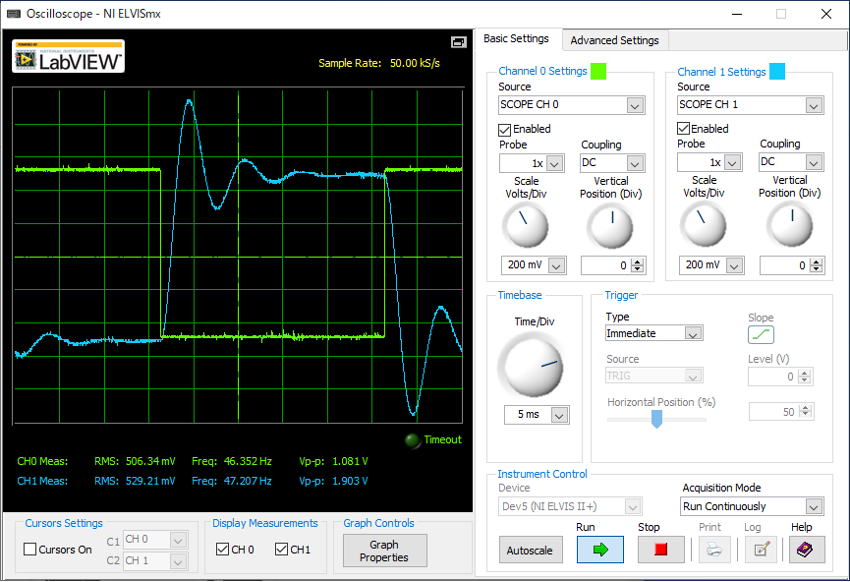
\includegraphics[width=0.8\linewidth]{src/figures/exp10/20k-low-sq.png}
		\subcaption{\SI{20}{k\ohm}でのバンドパスフィルタの出力波形}
	\end{subfigure}
	\caption{バンドパスフィルタの出力波形}
	\label{fig:exp10-band-sq}
\end{figure}


\clearpage
\subsection*{正弦波の周波数を変化させたときの出力波形}
\begin{figure}
	\centering
	\begin{subfigure}{0.8\linewidth}
		\centering
		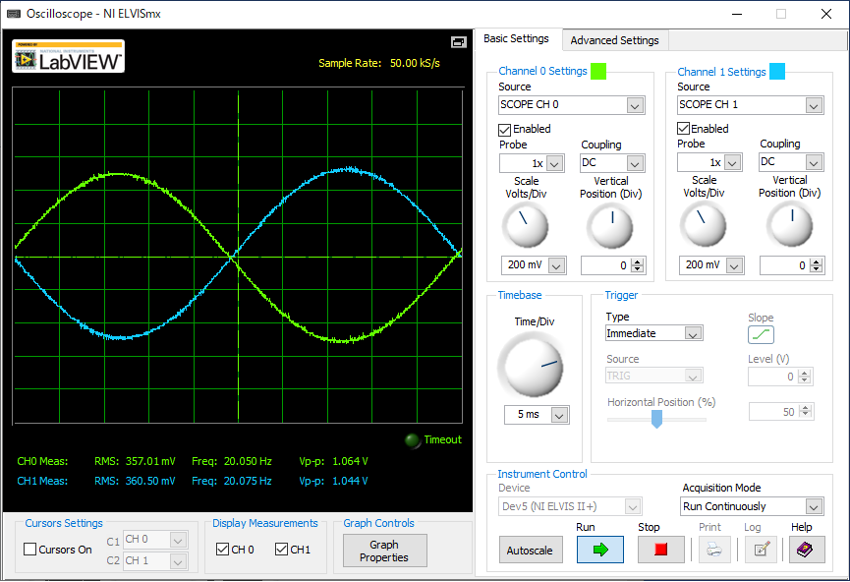
\includegraphics[width=0.8\linewidth]{src/figures/exp10/20k-20hz-sin.png}
		\subcaption{\SI{20}{Hz}}\label{fig:exp10-20hz}
	\end{subfigure}
	\begin{subfigure}{0.8\linewidth}
		\centering
		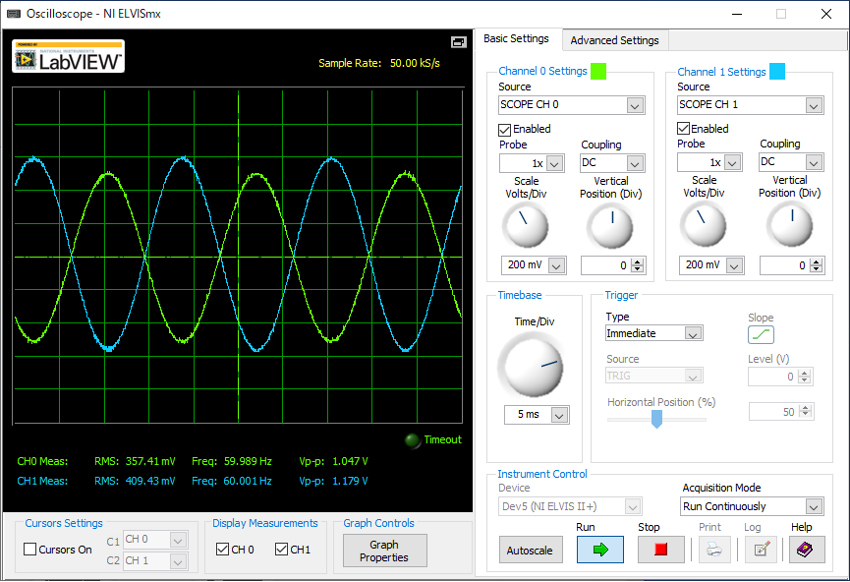
\includegraphics[width=0.8\linewidth]{src/figures/exp10/20k-60hz-sin.png}
		\subcaption{\SI{60}{Hz}}\label{fig:exp10-60hz}
	\end{subfigure}
\end{figure}
\begin{figure}
	\centering
	\begin{subfigure}{0.8\linewidth}
		\addtocontents{subfigure}{2}
		\centering
		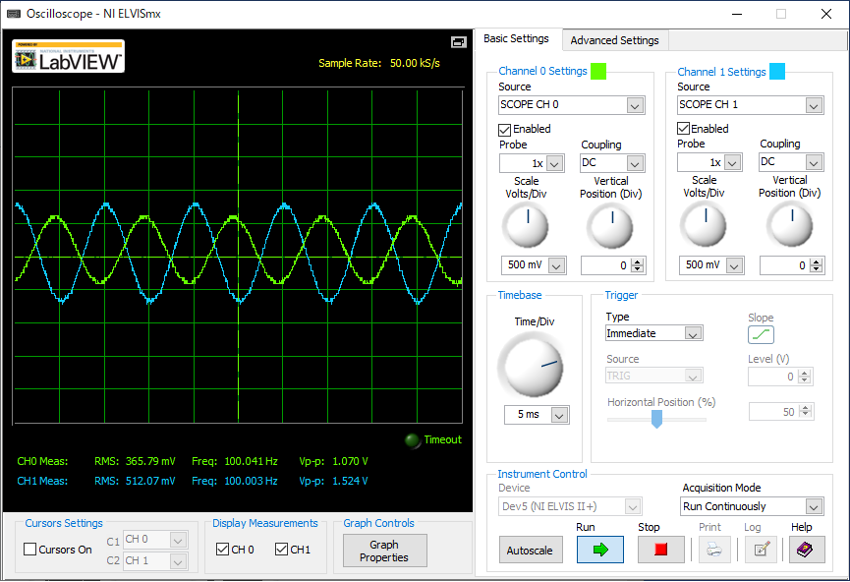
\includegraphics[width=0.8\linewidth]{src/figures/exp10/20k-100hz-sin.png}
		\subcaption{\SI{100}{Hz}}\label{fig:exp10-100hz}
	\end{subfigure}
	\begin{subfigure}{0.8\linewidth}
		\centering
		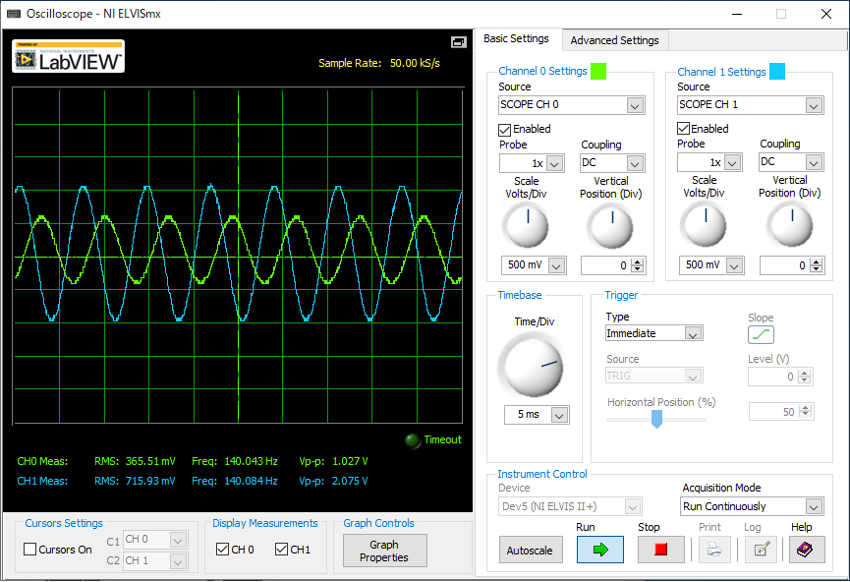
\includegraphics[width=0.8\linewidth]{src/figures/exp10/20k-140hz-sin.png}
		\subcaption{\SI{140}{Hz}}\label{fig:exp10-140hz}
	\end{subfigure}
\end{figure}
\begin{figure}
	\centering
	\begin{subfigure}{0.8\linewidth}
		\addtocounter{subfigure}{4}
		\centering
		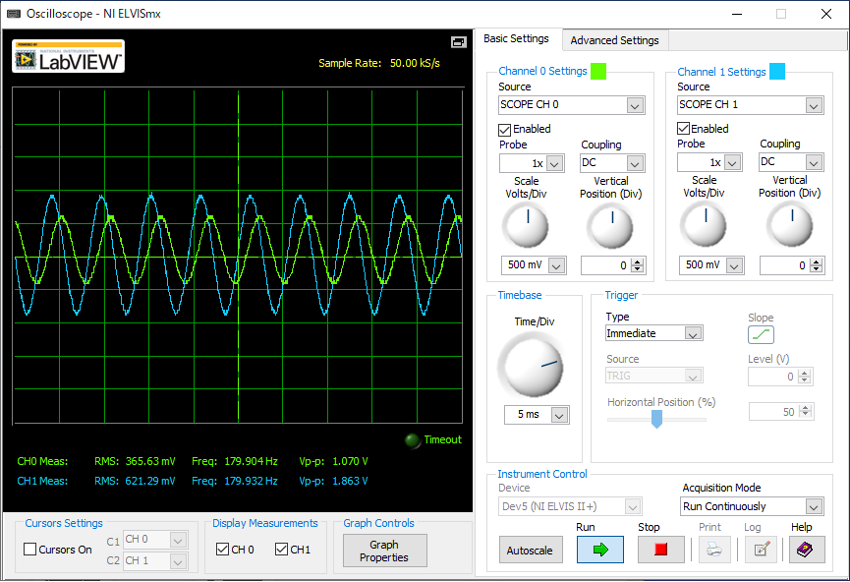
\includegraphics[width=0.8\linewidth]{src/figures/exp10/20k-180hz-sin.png}
		\subcaption{\SI{180}{Hz}}\label{fig:exp10-180hz}
	\end{subfigure}
	\caption{\SI{20}{Hz}から\SI{180}{Hz}まで\SI{40}{Hz}刻みで変化させたときの出力波形}\label{fig:exp10-band-sin}
\end{figure}




\end{document}
